\chapter{Implementation}
In order to achieve the project objective, it was necessary to apprehend a clear and unified understanding of how the different software components would interact with each other. The contributions made by this project should able to run alongside the existing project provided by AstaZero. To facilitate this, the application can be found in a file called ChalmersDemo.java~\cite{azGithubMobil} which is an Android activity that the user of the application can decide to navigate to. The user can easily navigate between these two implementations depending on the current use state. 

\section{Re-usability of existing software}
As previously mentioned in Sec.~\ref{AZ's app}, the AstaZero team had previously developed an Android application that could be utilized. The code is currently open-source, and contributions were made to the existing platform rather than creating a new one. As a result, certain code functions critical to the success of the project had already been created.

\subsection{IsoDrone}
To establish a connection between ATOS and the drone, the file IsoDrone~\cite{azGithubMobil} provides a Java class that can be initiated to create a drone object able to communicate over the ISO22133 protocol as presented in Sec.~\ref{ISO}. All test objects needs to report the status of the object every X seconds, decided in the ATOS configuration. The need to convert flight telemetry data into ISO-formatted strings were redundant, as this was already handled by the IsoDrone object. Instead, class variables could simply be changed to adjust current speed, heading, coordinates, and similar. The IsoDrone object then automatically transmitted this over the ISO22133 protocol to ATOS. 
\\ \\
Moreover, the protocol enabled the drone object to identify the current state of ATOS. This allowed the application to set up triggers that would activate when the state changed.

\subsection{Local coordinates to Latitude and Longitude}
Since ATOS worked with a local coordinate system, the location coordinates had to be converted to latitude and longitude coordinates in the Android application. The function handling the conversion was already present in the Waypoint1Activity file~\cite{azGithubMobil} and works by first reducing the amount of points and then creating a square matrix A with dimensions equal to the number of waypoints in the trajectory, and an array b with the same length as A's dimensions. It then populates A and b with values based on the trajectory information.
\\ \\
To find the radii for each waypoint, which will be used to define the radius of a circular area around each waypoint in which the drone will fly, the Android application utilizes LU decomposition. LU decomposition is a numerical method that decomposes a matrix into the product of two matrices: a lower triangular matrix (L) and an upper triangular matrix (U).
\\ \\
In the context of the waypoint conversion, LU decomposition is applied to the matrix A. By decomposing A into L and U, the Android application can efficiently solve the system of linear equations represented by the matrix equation $A * x = b$.
\\ \\
The LU decomposition allows for efficient solving of systems of equations, as it simplifies the process of finding the radii for each waypoint. Once the decomposition is performed, the solver can easily solve the equations for the radii, providing the necessary information to define the circular flight areas for the drone.
\\ \\
Finally, the method created parameters for each waypoint in the trajectory. It uses a method to convert the waypoint's Cartesian coordinates to geographic coordinates. It then sets various parameters, including the heading, altitude, and speed of the drone at each waypoint, as well as the radius calculated earlier.

\subsection{Ramer-Douglas-Peucker Algorithm} \label{douglas_puecker}
With the WaypointMission limitations presented in Sec.~\ref{sec:limit_WP}, the AstaZero team made use of the Ramer-Douglas-Peucker algorithm which is used for reducing the number of points in a curve while preserving its shape~\cite{Douglas1973ALGORITHMSCARICATURE}. This implementation made it possible to use trajectory files that normally would be composed of too many points to be run by the DJI WaypointMission software.  
\\ \\
The algorithm divides the line recursively, starting with a line segment between the first point and last one. The first and last points are automatically selected to be retained, it then identifies the point that is the maximum distance from the line segment. If the point is more than a predefined tolerance away from the line segment, it must be selected as a new start- and endpoint, otherwise the point can be discarded without impacting the shape of the curve. The algorithm recursively calls itself on the two newly created segments and the process is repeated for each new line segment until all the points are outside of the given tolerance. Fig.~\ref{fig:douglas_peucker} visualizes the algorithm. The result is a new curve with fewer points that still closely approximates the original one.
\\ \\
This algorithm was extensively employed in the deployment of curved trajectories to test objects that communicate over the ISO22133 protocol, primarily drones. However, it posed a challenge when deploying trajectories that only comprised points in a straight line, as it tended to reduce too many points. The subsequent section outlines a solution to this issue.

\begin{figure}[H]
    \centering
    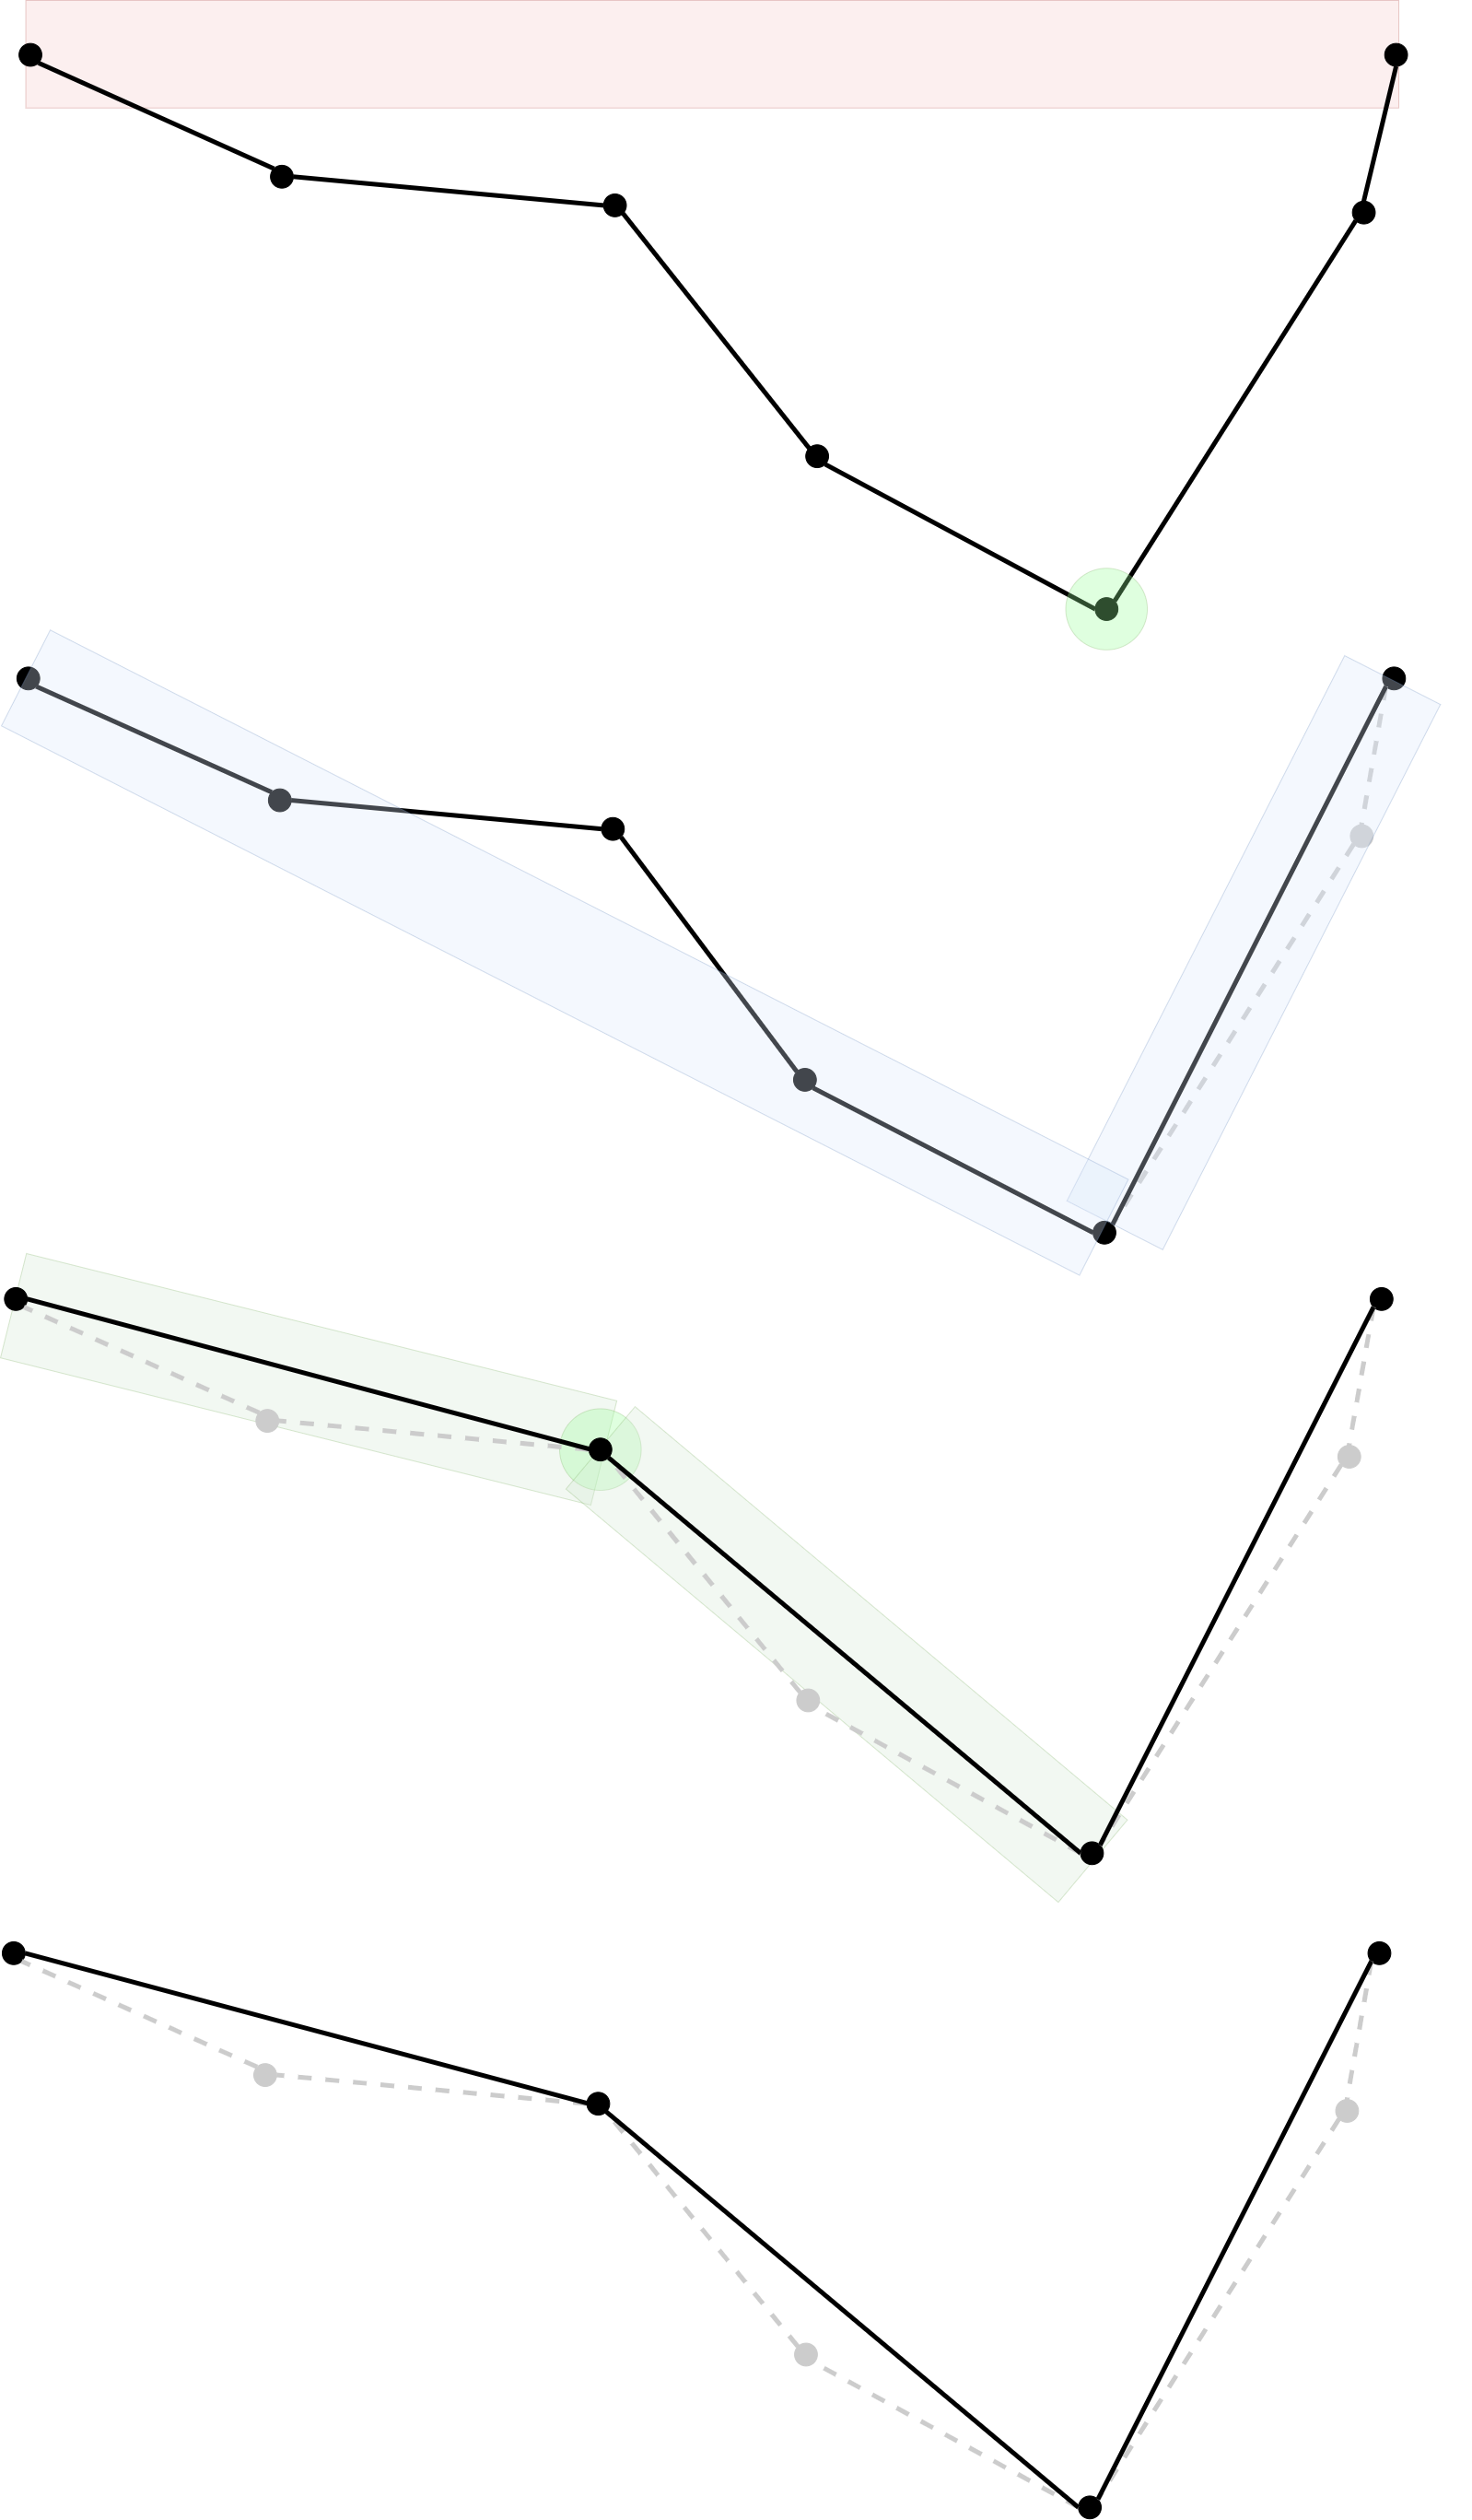
\includegraphics[scale=0.1]{figure/douglas_peucker_illustration.png}
    \caption{Illustration of the Ramer-Douglas-Peucker Algorithm. Source: Primary}
    \label{fig:douglas_peucker}
\end{figure}

\section{Addition to Ramer-Douglas-Puecker algorithm}
\label{sec:alt_douglas_peucker_algo}
The vast majority of the Ramer-Douglas-Puecker implementation produced by the AstaZero team was used with only minor modification and additions. The problematic aspect of the algorithm was that it reduced too many points when presented with a trajectory in a straight line, leaving too few\todo{tog bort to} points in the trajectory object to be sent to the next part of the point reduction implementation. The solution to this problem was to develop a simple collinearity check of the trajectory before applying the algorithm. In cases where all points in the trajectory lie on a straight line, the Ramer-Douglas-Peucker algorithm becomes overly complex and is therefore unnecessary. Moreover, adding a tolerance was deemed unnecessary as any straight segments in the programmatically generated trajectories would not deviate from the pre-defined path unless it was an intended curvature. Consequently, adding a tolerance would only introduce unnecessary complexity.
\newline

The algorithm's addition functioned by extracting the first two points of the input to establish a reference line for all subsequent points. Thereafter, one of the algorithm's loops was employed to iterate through each point in the input. During each iteration, if the cross product of the vector generated by the first and current points and the reference line equaled zero, the current point was determined to be collinear with the reference line. This calculation was done for every point in the input trajectory and if any resulting vector from the current point would fail to produce a cross product equal to zero, a \textit{isCollinear} variable is set to false. This would disable the superseding of the Ramer-Douglas-Puecker algorithm and allow it to run as intended. Algorithm~\ref{DP_code} describes the addition to the Ramer-Douglas-Puecker algorithm in pseudocode. 
\\ \\
\begin{algorithm}[H]
\caption{Pseudocode of the addition to the existing Ramer-Douglas-Peucker algorithm}\label{DP_code}
\SetAlgoLined
\SetKwFunction{douglasPuecker}{douglasPuecker}
\SetKwProg{Fn}{Function}{:}{}
\Fn{\douglasPuecker{$traj$, $resultTraj$}}{
    $**Algorithm\ starts**$\;
    \If{size of $traj$ < 3}{
        \Return $traj$\;
    }
    $isColinear \gets true$\;
    $x1, y1 \gets traj[0]$\;
    $x2, y2 \gets traj[\text{size of traj} - 1]$\;
    \For{$i \gets 1$ \KwTo\ size of $traj$}{
        $**First\ part\ of\ Ramer\ Douglas\ Peucker\ algorithm\ runs**$\;
        $px, py \gets traj[i]$\;
        $crossProduct \gets (x2 - x1) \cdot (py - y1) - (y2 - y1) \cdot (px - x1)$\;
        \If{$crossProduct \neq 0$}{
            $isColinear \gets false$\;
        }
        $**Original\ Ramer\ Douglas\ Peucker\ algorithm\ continues**$\;
    }
    \If{size of $traj$ > max number of points \textbf{\textup{and}} isColinear}{
        $multiplier \gets \lfloor \frac{\text{size of } traj}{\text{max number of points}}\rfloor$\;
        \For{$i \gets 0$ \KwTo\ size of $traj$-1}{
            $resultTraj \gets resultTraj + [traj[i]];$\;
            $i \gets i + multiplier;$\;
        }
        $resultTraj \gets resultTraj + traj[\text{size of traj}]$\;
        \Return $resultTraj$\;
    }
}
\end{algorithm}


\section{Main Activity} \label{sec:chalmers_demo_activity}
As stated in Sec.~\ref{Java, Android....}, activities are the basic building blocks of any Android application, including the AstaZero application. Each activity in the provided application represents a unique screen with its own graphical user interface, consisting of various elements like buttons, text views, images, and input fields. Every activity is responsible for managing its own tasks, such as establishing a connection between a remote controller and a drone. 
\\

The utilized approach facilitated the creation of a custom activity, named ChalmersDemo.java, which comprises the majority of the code employed in this project. Accompanying ChalmersDemo.java, an associated XML file, activity\_chalmers\_demo, contained all the visual details for the activity, as presented in the subsequent section. This approach ensured that the code provided by AstaZero for other functionalities remained unaffected, as it has its own activities.

\section{Graphical user interface} \label{sec:implement_GUI}
The GUI was developed continuously during the project, going through different iterations. The goal with the GUI was to make it as easy and as intuitive as possible, limiting the number of buttons and information shown on the screen, seen in Fig.~\ref{fig:GUI_v1}. The relevant information was determined to be:\\

\begin{itemize}
    \item The video feed of the camera with detected objects highlighted
    \item Latitude, longitude and altitude
    \item Drone state
    \item Mission information
    \item IP address of the phone
    \item Buttons for starting, stopping, landing and resetting the missions
\end{itemize}
%%https://developer.android.com/develop/ui/views/layout/relative
\begin{figure}[!h]
    \centering
    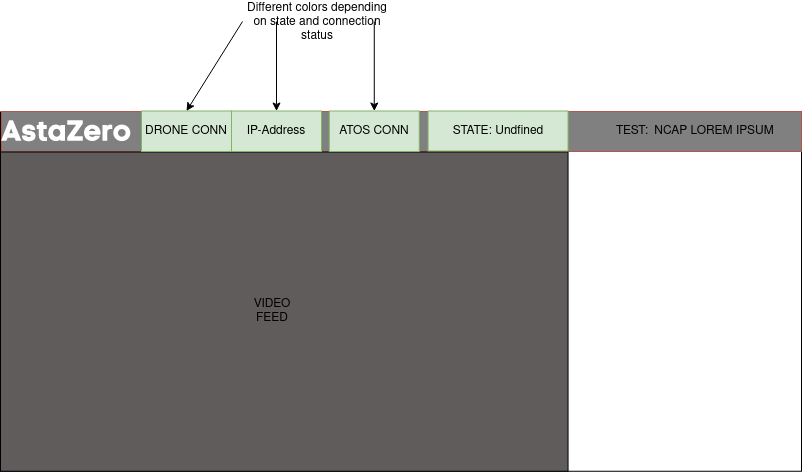
\includegraphics[width=\textwidth]{figure/v_1.2_GUI_demo_app.png}
    \caption{The first design idea for the GUI. Source: Primary}
    \label{fig:GUI_v1}
\end{figure}
This was implemented using XML and relies on a RelativeLayout hierarchy that contains different views as can be seen in the project \cite{azGithubMobil}. 
\newline

The GUI implementation was developed using two different strategies. The initial strategy was to create two separate applications, one for object tracking   and another for receiving trajectory data and flying the drone. This was quickly merged into one development process and went through different iterations, while maintaining the general layout. Parts were added and removed as the knowledge base increased with continuous input from the client, ultimately resulting in the final version of the GUI as presented in \ref{res: GUI}.

\section{DJI Flight Controller} \label{sec:DJI_flight_controll}
The flight aspect of the project is one of two main parts, the other one being object tracking presented in Sec.~\ref{sec:object_track}.

\subsection{Updates from the flight controller}
As presented in Sec.~\ref{Java, Android....}, the Android application makes heavy use of DJI's mobile SDK as it is the primary way for third-party software to interact with the drone. The foundation of this interaction is built upon the flight controller object~\cite{dji_flightcontroller} which facilitated the interaction between the drone's different flight-enabling systems. 
\newline

The DJI SDK constructor was used to initialize the flight controller, and a callback function for the controller was specified at the same time. This callback function provided the application with relevant information on every update, which occurred 10 times per second. This information included the drone's GPS position in terms of latitude and longitude, the strength of the GPS signal, and the current altitude. During the callback, a method was called to update the IsoDrone's flight data. This method utilized the flight controller object multiple times in various ways. One of its primary uses was to create, deploy, and activate WaypointMissions. The update flight data method also integrated ATOS into the Android application. An illustration of ATOS integration is provided in Fig.~\ref{fig:drone-flow}.

\begin{figure}[H]
    \centering
    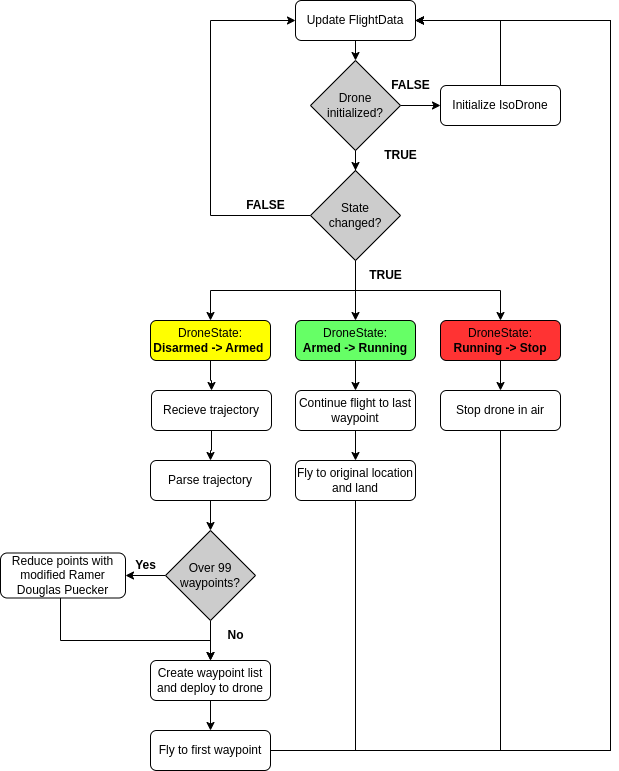
\includegraphics[scale=0.45]{figure/Flowchart-drone.png}
    \caption{Flight data update flow chart. Source: Primary}
    \label{fig:drone-flow}
\end{figure}

When the state of the IsoDrone changes from Disarmed to Armed, the trajectory is passed through the application and verified to be in the right format, as can be seen in Fig.~\ref{fig:drone-flow}. If the trajectory is too large, it is reduced by the algorithm described in Sec. ~\ref{douglas_puecker} and Algorithm~\ref{DP_code}. When the trajectory is correct, the application transforms the trajectory into global latitudinal and longitudinal coordinates through a coordinate conversion script developed by AstaZero. The application then transmits the trajectories to the drone via a DJI protocol from the remote controller connected to the Android device and the drone flies to the first waypoint. At the first waypoint, the drone stops and hovers in its place. Following this, the test commences when the ATOS state is changed to ``Running'', and the drone as well as all other test objects execute their pre-determined paths. 

\subsection{Updating the GUI} \label{sec:updating_UI}
Updating the user interface was crucial for providing real-time information about the drone's location, altitude, and GPS signal strength as well as showing the test track personnel what is currently being filmed. The GUI had to be updated continuously, and this was achieved by also sending information to the GUI when receiving the callback presented in Sec.~\ref{sec:DJI_flight_controll}. The GUI also used information such as IP address and ATOS state from the IsoDrone object, as well as the current waypoint the drone is flying towards. This facilitated the real-time updates needed by the drone operator to make sure the application and drone was running the way it was intended to be run.

\section{Object detection} \label{sec:image_rec}
Object detection was only implemented using the mobile camera and not the drone camera due to a couple of obstacles described in Ch.~\ref{sec:discussion}.
\\ \\
As mentioned in Sec.~\ref{sec:Obj_detextion}, TensorFlow Lite was used for object detection in the project, mainly because it had the fast classification that was needed during the test. The image recognition is heavily inspired by an open source project~\cite{githubTensorFlowApp} that uses a TensorFlow Lite model to recognize objects. 
\\ \\
The application utilized a pre-trained SSD model which uses the convolutional layers of MobileNet v.1.0. The ssd\_mobilenet\_v1\_coco model~\cite{TensorFlow2021TensorFlowZoo} was selected and is visualized in \ref{Apend:object_detect_model_1} and \ref{Apend:object_detect_model_2}. As described in Sec.~\ref{ssdbackground}, an SSD offers computational efficiency while retaining competitive accuracy, making it a perfect fit for a real-time object detection running on a mobile device. Despite the model looking intricate and excessively detailed, the number of parameters is relatively low for the task at hand. The model uses convolutions layers to reduce the number of parameters compared to alternative models such as the Inception V2 and VGG16\cite{mobilenet} which uses 10 million and 14 million parameters respectively. The MobileNet only uses 3.2 parameters. The relatively low amount of parameters enhances the speed of the model, making it the best fit for the task at hand~\cite{cnnforklarning}.
\\ \\
The last part of the model's name, ''coco'', implies that the model has been trained on the COCO dataset~\cite{COCOConsortiumCommonContext}. The COCO dataset is a free website which provides over 200 thousand labeled images to train models on. The model used is able to detect around 90 objects, including persons, cars, bicycles and many more. The selection of this particular model was based on its ability to detect a wide variety of objects, thus rendering it versatile in numerous situations. The Euro NCAP test comprises evaluations where the objects to be detected could be other than cars, including trucks and bicycles. Having a model that can recognize diverse objects offers the test operator the liberty to track any object on the premises with minimal code modifications.
\\ \\
The camera feed from the mobile device was transmitted to the application in a RAW format, which is an unprocessed image data format~\cite{Menasco2022MethodFormat}, and subsequently decoded and displayed on the screen. As the video was displayed, a frame from the feed was simultaneously sent to be processed in the background and converted from RAW to RGBA format in a bitmap. The RGBA color model is a three-channel, red-green-blue color representation enriched by an additional alpha channel~\cite{Menasco2022MethodFormat}. This transformation was necessary because the chosen model required the input image to be in the RGBA format.
The model output has different attributes for each detected object, which are:\\
\begin{enumerate}\itemsep0.3pt
    \item Index - The index of the identified object
    \item Label - The type of the object
    \item Confidence - How sure the model is about the predicted object, 0-100\,\%
    \item Rectangle - Coordinates for drawing a rectangle over the detected object\\
\end{enumerate}
Since the tests would be conducted in controlled conditions with only a few other objects, several tests were carried out and a confidence threshold value of 50\% was found to be optimal.
\\ \\
Consequently, the model was configured to detect people and cars only, and the results were filtered to display only the detected instances of these objects. However, if there arises a requirement to detect other types of objects, such as trucks or buses, the code can be easily modified accordingly. If an object was detected with a confidence score lower than the threshold, it was ignored. As the function iterated through the detected objects, it also annotated the video stream with labeled rectangles and their respective confidence scores. An illustration describing the image recognition process can be seen in Fig.~\ref{fig:Objectdetection-flowchart}.

\begin{figure}[H]
    \centering
    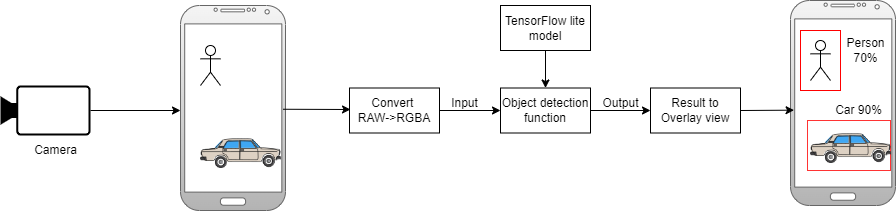
\includegraphics[scale=0.45]{figure/object_detection_illustration.png}
    \caption{Flowchart describing the object detection sequence. Source: Primary}
    \label{fig:Objectdetection-flowchart}
\end{figure}

\section{Object tracking} \label{sec:object_track}
As previously mentioned in Sec.~\ref{Tracking algorithm}, object tracking needs to be implemented with the use of object detection to track chosen vehicle. But as stated in the previous section, object detection is only implemented on the mobile camera and not the drone camera, where the object tracking algorithm was supposed to be. Since the adjustments needed for the tracking algorithm relied on the movement of the camera gimbal, it was decided to not pursue a solution until the object detection algorithm was fully functional on the drone camera.
 

